\documentclass{scrreprt}

\usepackage{aligned-overset}
\usepackage{amsmath}
\usepackage{amsthm}
\usepackage{amssymb}
\usepackage{bm}
\usepackage[inline, shortlabels]{enumitem}
\usepackage{hyperref}
\usepackage[utf8]{inputenc}
\usepackage{listings}
\usepackage{multicol}
\usepackage{mathtools}
\usepackage{pdflscape}
\usepackage{physics}
\usepackage{polynom}
\usepackage{tabularx}
\usepackage[table]{xcolor}
\usepackage{titling}
\usepackage{fancyhdr}
\usepackage{xfrac}
\usepackage{pgfplots}

\pgfplotsset{compat = newest}
\usepgfplotslibrary{fillbetween}
\usetikzlibrary{arrows, arrows.meta}
\usetikzlibrary{calc}
\usetikzlibrary{patterns}

\author{Karsten Lehmann}
\date{WiSe 2024/25}
\title{Übungsblatt 12\\INF-B-110, Diskrete Strukturen}

\setlength{\parindent}{0pt}

\setlength{\headheight}{26pt}
\pagestyle{fancy}
\fancyhf{}
\lhead{\thetitle}
\rhead{\theauthor}
\lfoot{\thedate}
\rfoot{Seite \thepage}

\newcommand{\ggT}[0]{\text{ggT}}
\DeclarePairedDelimiter{\floor}{\lfloor}{\rfloor}

\begin{document}

\paragraph{Ü 12.1}
\begin{enumerate}[(a)]
\item Auf der Menge $A = \qty\big{1, 2, 3, 4, 5, 6, 7, 8, 9}$ ist folgende
  Relation gegeben:
  \[
    R = \qty\big{
      \qty\big(a, a)
      \:{\big|}\:
      a \in A
    } \cup \qty\big{
      \qty\big(1, 9),
      \qty\big(2, 4),
      \qty\big(2, 5),
      \qty\big(2, 7),
      \qty\big(3, 6),
      \qty\big(4, 2),
      \qty\big(4, 5),
      \qty\big(4, 7),
      \qty\big(5, 2),
      \qty\big(5, 4),
      \qty\big(5, 7),
      \qty\big(6, 3),
      \qty\big(7, 2),
      \qty\big(7, 4),
      \qty\big(7, 5),
      \qty\big(9, 1)
    }
  \]
  \begin{enumerate}[(1)]
  \setcounter{enumii}{1}
  \item Zeichnen Sie ein Diagramm des Graphen $G = \qty\big(V, E)$ mit $V = A$
    und der Kantenmenge $E = \qty{
      \qty\big{a, b} \in A \times A
      \:\middle|\:
      a \ne b,
      \qty\big(a, b) \in R
    }$

    \subparagraph{Lsg.} \phantom{\null}

    \begin{tikzpicture}
      \node[circle, draw, inner sep=0pt, minimum size=1mm,label=above:{1}] (1) at (0,0) {};
      \node[circle, draw, inner sep=0pt, minimum size=1mm,label=above:{9}] (9) at (-1,-0.5) {};

      \node[circle, draw, inner sep=0pt, minimum size=1mm,label=left:{2}] (2) at (-1,-2) {};
      \node[circle, draw, inner sep=0pt, minimum size=1mm,label=above:{4}] (4) at (0.5,-1) {};
      \node[circle, draw, inner sep=0pt, minimum size=1mm,label=right:{5}] (5) at (0,-2) {};
      \node[circle, draw, inner sep=0pt, minimum size=1mm,label=below:{7}] (7) at (0.5,-3) {};

      \node[circle, draw, inner sep=0pt, minimum size=1mm,label=above:{3}] (3) at (0,-4) {};
      \node[circle, draw, inner sep=0pt, minimum size=1mm,label=above:{6}] (6) at (-1,-3.5) {};

      \node[circle, draw, inner sep=0pt, minimum size=1mm,label=above:{8}] (8) at (2,-2) {};

      \draw (1) -- (9);
      \draw (2) -- (4) -- (5) -- (7) -- (2) -- (5);
      \draw (4) -- (7);
      \draw (3) -- (6);


    \end{tikzpicture}

  \setcounter{enumii}{0}
  \item Zeigen Sie, dass $R$ eine Äquivalenzrelation ist.
    Geben Sie die Äquivalenzklassen von $R$ und die durch $R$ erzeugte
    Partition von $A$ an.

    \subparagraph{Lsg.} Eine Äquivalenzrelation ist eine Relation, die
    \emph{reflexiv}, \emph{symmetrisch} und \emph{transitiv} ist.
    Nun ist $R$ offensichtlich \emph{reflexiv}, da
    $\qty{\qty\big(a, a) \:\middle|\: a \in A} \in R$.

    Weiter ist $R$ auch \emph{symmetrisch}, es lásst sich schnell erblicken, dass
    für alle $\qty\big(a, b) \in R$ auch $\qty\big(b, a) \in R$.

    Schließlich ist $R$ auch \emph{transitiv}, da der Graph aus Teilaufgabe
    (a)(2) eine disjunkte Vereinigung vollständiger Graphen ist.

    Die Áquivalenzklassen von $R$ sind (oder die von $R$ erzeugte Partition auf
    $A$ ist)
    \begin{itemize}
    \item $1 / R = \qty\big{1, 9} = 9 / R$
    \item $2 / R = \qty\big{2, 4, 5, 7} = 4 / R = 5 / R = 7 / R$
    \item $3 / R = \qty\big{3, 6} = 6 / R$
    \item $8 / R = \qty\big{8}$
    \end{itemize}
  \end{enumerate}

\newpage
\item Zeigen Sie, dass die Relation $R \coloneqq \qty{
    \qty\big(z_1, z_2) \in \mathbb{C} \setminus \qty\big{0} \times
    \mathbb{C} \setminus \qty\big{0}
    \:\middle|\: z_1 \cdot \overline{z_2} \in \mathbb{R}
  }$ eine Äquivalenzrelation ist.
  Skizzieren Sie die Äquivalenzklasse $\qty\big(1 + i) / R$ in der Gaußschen
  Zahlenebenen.

  \subparagraph{Lsg.} Eine Äquivalenzrelation ist eine Relation, die
  \emph{reflexiv}, \emph{symmetrisch} und \emph{transitiv} ist.
  \begin{itemize}
  \item[\emph{reflexiv}:] Sei $z = \qty\big(a + bi) \in \mathbb{C}$.
    Dann ist $\qty\big(a + bi)\qty\big(a + bi) =
    \qty\big(a^2 + b^2) + \qty\big(-ab + ab)i
    = a^2 + b^2 \in \mathbb{R}$ und somit $\qty\big(a, a) \in R$.

    Damit ist $R$ \emph{reflexiv}.

  \item[\emph{symmetrisch}:] Seien $z_1, z_2 \in \mathbb{C}$ mit
    $z_1 \cdot \overline{z_2} \in \mathbb{R}$.
    Dabei ist zu wissen, dass die komplexe Konjugation ein selbstinverser
    (dass heißt $\overline{\ldots}^2 = \text{id}$) Gruppenisomorphismus der
    abelschen Gruppe $\qty{\mathbb{C}\setminus \qty\big{0}, \cdot}$ ist.
    Somit ist
    \begin{flalign*}
      z_1 \cdot \overline{z_2}
      \overset{\text{Selbstinvers}}&= \overline{\overline{z_1}} \cdot \overline{z_2} \\
      \overset{\text{Konjugation ist isomorph}}&= \overline{\overline{z_1} \cdot z_2} \\
      \overset{\text{abelsch}}&= \overline{z_2 \cdot \overline{z_1}} \\
      &= \overline{z_2} \cdot z_1 \\
      \overset{\text{Weil das Konjugierte in $\mathbb{R}$}}&\in \mathbb{R}
    \end{flalign*}

  \item[\emph{transitiv}:] Seien $z_1, z_2, z_3 \in \mathbb{C}$ mit
    $z_1 \cdot \overline{z_2} \in \mathbb{R}$ und
    $z_2 \cdot \overline{z_3} \in \mathbb{R}$.

    Dann ist
    \begin{flalign*}
      \underset{\in \mathbb{R}}{\underbrace{z_1 \cdot \overline{z_2}}} \cdot
      \underset{\in \mathbb{R}}{\underbrace{z_2 \cdot \overline{z_3}}}
      &= z_1 \cdot \overline{z_3} \cdot \underset{\in \mathbb{R}}{\underbrace{\abs{z_2}^2}} \in \mathbb{R}
    \end{flalign*}
    $\Rightarrow z_1 \cdot \overline{z_3} \in R$.
  \end{itemize}

  Sei $z = \qty\big(a + bi) \in \mathbb{C}$.
  Dann ist $\qty\big(a + bi) \cdot \qty\big(1 + i) =
  \qty\big(a + b) + \qty\big(a - b)i$.
  Somit ist $z$ in der Äquivalenzklasse von $1 + i$, genau dann wenn $a - b = 0$.

  \begin{tikzpicture}
    \begin{axis}[
      axis equal image,
      axis x line=center,
      axis y line=center,
      grid=both,
      xmin=-1.5,
      xmax=1.5,
      xtick distance=1,
      ymin=-1.5,
      ymax=1.5,
      ytick distance=1,
    ]
    \node[circle, draw, inner sep=0pt, minimum size=1mm,label=above:{$1 + i$}] at (1,1) {};

    \draw (-1.6, -1.6) -- (1.6, 1.6) node[midway, xshift=15, label=above right:{$\qty\big(1 + i) / R$}] {};
    \end{axis}
  \end{tikzpicture}

\newpage
\item Untersuchen Sie, für welche Graphen $G = \qty\big(V, E)$ die Relation
  \[
    R_G \coloneqq \qty{
      \qty\big(u, v) \in V^2
      \:\middle|\:
      \text{Es gibt einen Block, der sowohl $u$ als auch $v$ enthält}
    }
  \]
  eine Äquivalenzrelation ist.

  \subparagraph{Lsg.} Die Eigenschaften \emph{reflexiv} und \emph{symmetrisch}
  sind hier klar.
  Betrachten wir die Eigenschaft \emph{transitiv}: Seien $B_1$, $B_2$ Blöcke mit
  $v \in V\qty\big(B_1) \cap V\qty\big(B_2)$.

  \begin{tikzpicture}
    \node[circle, draw, inner sep=0pt, minimum size=2cm] at (0, 0) {$B_1$};
    \node[circle, draw, inner sep=0pt, minimum size=2cm] at (1.5, 0) {$B_2$};

    \node[circle, draw, inner sep=0pt, minimum size=1mm,label=above:{$v$}] at (0.75,0) {};
    \node[circle, draw, inner sep=0pt, minimum size=1mm,label=above:{$u$}] at (-0.5,-0.35) {};
    \node[circle, draw, inner sep=0pt, minimum size=1mm,label=above:{$w$}] at (2,0.2) {};
  \end{tikzpicture}

  Dann ist $\qty\big(u, v) \in R$ und $\qty\big(w, v) \in R$, allerdings nicht
  $\qty\big(u, w) \in R$.
  Somit ist die Relation eine Äquivalenzrelation, falls $G$ eine disjunkte
  Vereinigung von Blöcken ist.
\end{enumerate}

\paragraph{Ü 12.2} Auf der Menge $A \coloneqq \qty\big{2, \ldots, 9}$ ist die
Relation $R \coloneqq \qty{
  \qty\big(x, y) \in A^2
  \:\middle|\: x \mod y = 0
}$ definiert.
\begin{enumerate}[(a)]
\item Geben Sie $R$ als Menge von Paaren an.

  \subparagraph{Lsg.}
  \[
    R = \qty{
      \qty\big(2, 2),
      \qty\big(3, 3),
      \qty\big(4, 2),
      \qty\big(4, 4),
      \qty\big(5, 5),
      \qty\big(6, 2),
      \qty\big(6, 3),
      \qty\big(6, 6),
      \qty\big(7, 7),
      \qty\big(8, 2),
      \qty\big(8, 4),
      \qty\big(8, 8),
      \qty\big(9, 3),
      \qty\big(9, 9)
    }
  \]

\item Ist $R$ eine Quasiordnung?
  Ist $R$ eine partielle Ordnung?

  \subparagraph{Lsg.} Eine Quasiordnung ist eine Relation, die sowohl
  \emph{reflexiv} als auch \emph{transitiv} ist.

  Nun ist die Eigenschaft \emph{reflexiv} offensichtlich.
  Seien nun $a, b, c \in A$, dann gilt
  $a|b \land b|c \Rightarrow a|c$.
  Somit ist $R$ auch \emph{transitiv} und eine Quasiordnung.

  \textbf{Lemma:} Sei $\leq$ eine partielle Ordnung auf $A$.
  \begin{enumerate}[(1)]
  \item Sei $A' \subseteq A$.
    Dann ist $\leq \cap \qty\big(A' \times A')$ eine partielle Ordnung auf $A$
  \item $\geq$ ist eine partielle Ordnung auf $A$, mit
    $\geq = \qty{
      \qty\big(a, b) \in A
      \:\middle|\:
      \qty\big(b, a) \in \leq
    }$.
  \end{enumerate}
  Nun ist $|$ bereits eine partielle Ordung auf $\mathbb{N}$ und da
  $A \subseteq \mathbb{N}$ auch $R$ eine partielle Ordnung.
\end{enumerate}

\newpage
\paragraph{Ü 12.3} Für eine endliche Menge $A \ne \emptyset$ und eine Abbildung
$f \colon A \to A$ wird die Relation
\[
  R_f \coloneqq \qty{
    \qty\big(a, b) \in A^2
    \:\middle|\:
    \exists n \in \mathbb{N} \colon b = f^n\qty\big(a)
  }
\]
betrachtet.
(Dabei ist $f^n$ die $n$-malige Hintereinanderausführung von $f$,
$f^0 = \text{id}$)
\begin{enumerate}[(a)]
\item Zeigen Sie, dass $R_f$ eine Quasiordnung ist.

  \subparagraph{Lsg.} Es ist $\qty\big(a, a) \in R_f$, da $a = f^0\qty\big(a)$.
  Somit ist $R$ \emph{reflexiv}.

  Seien weiter $b = f^n\qty\big(a)$ und $c = f^m\qty\big(b)$.
  Dann ist $c = f^{n + m}\qty\big(a)$ und $R$ somit \emph{transitiv}.

\item Zeigen Sie, dass $R_f$ für $f \colon \mathbb{Z}_5 \to \mathbb{Z}_5$,
  $f\qty\big(a) \coloneqq a^2 + 1 \qty\big(\mod 5)$ keine partielle Ordnung ist.
  Bestimmen Sie die zu $R_f$ gehörige Faktorordnung $\leq$ auf $A / \sim$ mit
  \[
    \sim \coloneqq \qty{
      \qty\big(a, b) \in A^2
      \:\middle|\:
      \qty\big(a, b) \in R_f, \qty\big(b, a) \in R_f
    }
  \]
  Zeichnen Sie ein Hassediagramm dieser Faktorordnung.

  \subparagraph{Lsg.} Als Quasiordnung ist $R_f$ bereits \emph{reflexiv} und
  \emph{transitiv}.
  Wäre nun $R_f$ eine partielle Ordnung, dann wäre $R_f$ auch noch
  \emph{antisymmetrisch}.
  Somit ist zu zeigen, dass $R_f$ nicht \emph{antisymmetrisch} ist.

  Nun ist
  \begin{itemize}
  \item $f\qty\big(0) = 0^2 + 1 \equiv 1 \qty\big(\mod 5)$
  \item $f\qty\big(1) = 1^2 + 1 \equiv 2 \qty\big(\mod 5)$
  \item $f\qty\big(2) = 2^2 + 1 \equiv 0 \qty\big(\mod 5)$
  \item $f\qty\big(3) = 3^2 + 1 \equiv 0 \qty\big(\mod 5)$
  \item $f\qty\big(3) = 4^2 + 1 \equiv 2 \qty\big(\mod 5)$
  \end{itemize}
  und $0 = f\qty\big(2)$ sowie $2 = f^2\qty\big(0)$, aber $0 \ne 2$.
  Damit ist $R_f$ nicht \emph{antisymmetrisch} und keine partielle Ordnung.

  Nun zur Faktorordnung
  \[
    \begin{array}{c}
      a/\sim \leq b/\sim \\
      \Updownarrow \\
      a \preceq b \\
      \Updownarrow \\
      \exists n \in \mathbb{N} \colon b = f^n\qty\big(a)
    \end{array}
  \]
  Als Diagramm

  \begin{tikzpicture}
    \node[circle, draw, inner sep=0pt, minimum size=1mm,label=above:{$\qty\big{0, 1, 2}$}] (1) at (0,0) {};
    \node[circle, draw, inner sep=0pt, minimum size=1mm,label=below left:{$\qty\big{3}$}] (2) at (-0.5,-1) {};
    \node[circle, draw, inner sep=0pt, minimum size=1mm,label=below right:{$\qty\big{3}$}] (3) at (0.5,-1) {};

    \draw (3) -- (1) -- (2);
  \end{tikzpicture}
\end{enumerate}
\end{document}
